\chapter{Indirekte Fernlokalisierung mit IEEE 802.11}
\label{ch:phase1}
Bei der indirekten Fernlokalisierung wird die Messgröße auf der mobilen Einheit gemessen.
Die Ortungsinformation wird dann implizit durch versenden der gemessenen Werte oder explizit durch versenden der berechneten Position an den Ortungsserver übermittelt.
Wird IEEE 802.11 verwendet muss die mobile Einheit mit einem Access Point assoziiert um Informationen an den Ortungsserver übermitteln zu können.
Eine Lösung zur indirekten Fernlokalisierung muss deshalb mindestens auf Protokollebene vier des OSI-Modells arbeiten.
Für die Übermittelung steht ein WLAN-Netzwerk zur Verfügung.

\begin{figure}[h]
  \centering
	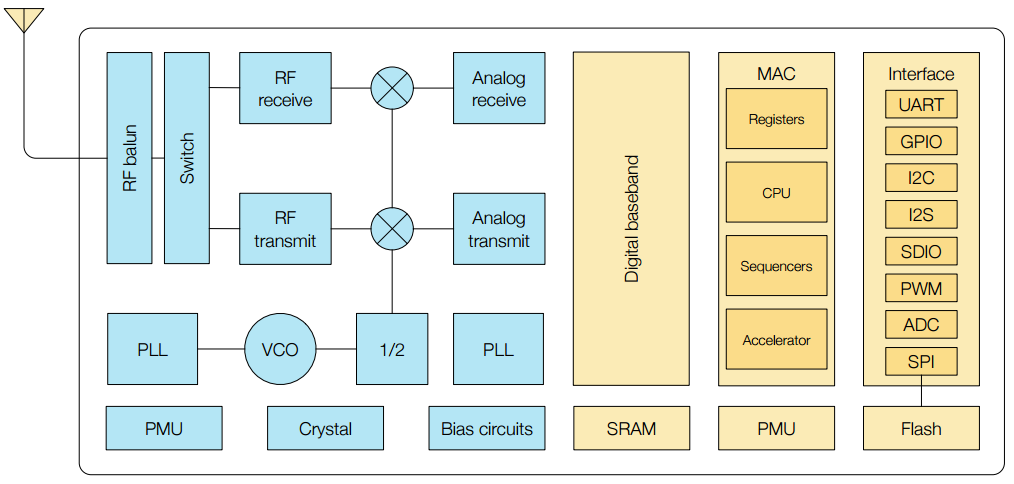
\includegraphics[width=\textwidth]{images/espblock.png}
  \caption{Blockdiagramm des ESP8266, aus \cite{espressif2017esp8266}}
  \label{fig:espblock}
\end{figure}

\section{ESP8266}
Der ESP8266 soll als Hardware für das Tag eingesetzt werden, dabei handelt es sich um einen Microcontroller von Espressif.
Der ESP8266 besitzt neben einer CPU eine 802.11b/g/n"-/e/i-fähige WLAN-Einheit und beherrscht diverse andere, kabelgebundene Kommunikationsstandards wie zum Beispiel GPIO, I2C und SPI, siehe Abbildung \ref{fig:espblock}. \\
Da der ESP8266 selbst weder über Flashspeicher, noch über eine Antenne verfügt wird er auf einem Modul mit diesen Komponenten verbaut. 
Die in dieser Arbeit betrachteten Module sind das ESP-12S und das ESP-12F.
Das neuere ESP-12F sollte eine höhere Reichweite bei der Funkübertragung entfalten, dies wird noch Gegenstand eines Experiments sein.
%TODO Antennen markieren
Abbildung \ref{fig:espmodules} zeigt die beiden Module nebeneinander, die unterschiedlichen Antennenformen sind deutlich zu erkennen.\\
Espressif gibt im Datenblatt auch Aufschluss über den Energieverbrauch des ESP8266, siehe dazu Tabelle \ref{table:esppower}.
Für die Prototypenentwicklung wird ein ESP-12S Modul auf einem Adafruit Feather Huzzah verwendet, dieses stellt mit dem CP2104 eine serielle Verbindung zum ESP her, reguliert die Spannung für das Modul auf 3,3V und bringt den 2mm Pinabstand des ESP-12S Moduls auf die für Breadboards üblichen 2,5mm.
Das Adafruit Feather Huzzah ESP8266 mit ESP-12S ist in Abbildung \ref{fig:espmodules} links abgebildet.

\begin{figure}[h]
  \centering
	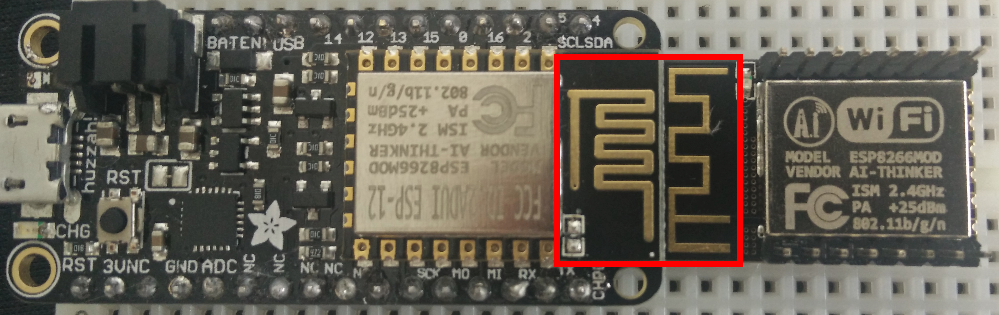
\includegraphics[width=\textwidth]{images/espmodules.png}
  \caption{Vergleich der Antennen (im rot markierten Bereich), links: ESP12-S verbaut auf einem Adafruit Feather Huzzah, rechts: ESP12-F.}
  \label{fig:espmodules}
\end{figure}

\begin{table}[h]
  \centering
  \caption{Energieverbrauch des ESP8266 bei verschiedenen Operationen, aus \cite{espressif2017esp8266}}
	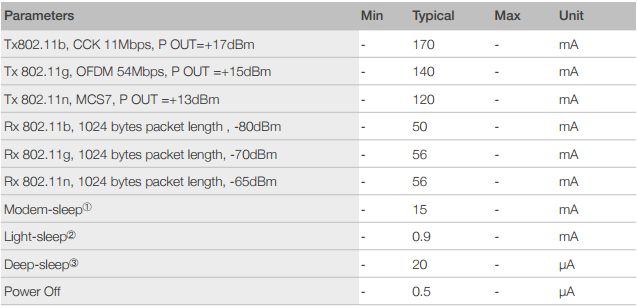
\includegraphics[width=\textwidth]{images/esppower.png}

  \label{table:esppower}
\end{table}


\subsection{ESP8266 Arduino Core}
Eine einfache Möglichkeit den ESP8266 zu programmieren stellt die bekannte Arduino IDE dar \cite{banzi2017arduino}.\\
Unter Windows muss zunächst der Treiber für den \textit{CP2104 USB-to-Serial Chip} installiert werden, auf Linux und Mac entfällt dieser Schritt \cite{fried2017feather}.
Nach der Installation der Arduino IDE muss dort in den Einstellungen unter \textit{Additional Boards Manager URLs} die URL \url{http://arduino.esp8266.com/stable/package_esp8266com_index.json} hinzugefügt werden.  
Nach einem Neustart der IDE kann im \textit{Boards Manager} das Paket für den ESP8266 heruntergeladen werden und anschließend das Board \textit{Adafruit HUZZAH ESP8266} ausgewählt werden. \\
Ist das Board über USB mit dem Computer verbunden, kann nun eigener Code oder eines der Beispiele aus \textit{Examples for Adafruit HUZZAH ESP8266} mit STRG+U auf den ESP geladen werden. 
Dieser Vorgang wird im Folgenden als \emph{flashen} bezeichnet. \\
Der ESP8266 Arduino Core wird als Open Source Projekt gepflegt und setzt die ESP Open SDK auf einen, für die Arduino IDE üblichen Stil um \cite{arduino2017core}. 
Dabei wird möglichst die Kompatibilität zu Arduino gewahrt, das führt oft dazu, dass bereitgestellte Funktionen der SDK nicht in Arduino umgesetzt wurden.
Sollten die Funktionen dennoch benötigt werden, können die Header-Dateien der SDK direkt importiert werden:

\begin{verbatim}
//Hier wird ein Header des ESP8266 Arduino Core importiert
#include <ESP8266WiFi.h> 

//Hier wird ein Header der ESP Open SDK importiert
extern "C" {#include "user_interface.h"} 
\end{verbatim}

Der ESP8266 Arduino Core wurde in der Version 2.3.0 verwendet.

\subsection{ESP Open SDK}
Statt mit der Arduino Core Umsetzung der ESP Open SDK kann natürlich auch direkt mit ihr programmiert werden \cite{esp2017open}. \\
Dazu muss zunächst das Github Projekt geklont werden: \texttt{git clone --recursive \url{https://github.com/pfalcon/esp-open-sdk}.git} und anschließend mit \texttt{make} kompiliert werden.
Wurde die Kompilierung erfolgreich abgeschlossen, sollte die Pfadvariable (PATH) entsprechend der Meldung des make-Tools erweitert werden. \\
Die in C geschriebenen Programme können nun mit einem modifizierten GCC-Kompiler kompiliert und anschließend mit dem esptool.py zunächst in ein Image umgewandelt und dann geflasht werden. 
Das in \textit{examples} enthaltene \textit{blinky} Beispiel beinhaltet neben dem Beispielcode eine Makefile, in der diese Schritte nachvollzogen werden können, mit \texttt{make flash} wird das Beispiel kompiliert und \emph{geflasht}. \\
Programme werden in regulärem C unter Zuhilfenahme der in \texttt{/sdk/include} enthaltenen Header-Dateien geschrieben, zu beachten ist nur, dass einige Funktionen der \texttt{stdlib.h} nicht verwendet werden können.
Dies betrifft vor allem direkten Speicherzugriff wie zum Beispiel \texttt{memcpy}, hier muss stattdessen \texttt{os\_memcpy} verwendet werden.
Alle betroffenen Funktionen sind in \texttt{osapi.h} beschrieben. \\
Einige frühe Experimente zeigten, dass Programme, die mit der ESP Open SDK geschrieben wurden auf dem ESP8266 schneller starten als solche, die mit dem ESP8266 Arduino Core geschrieben wurden.
Diese Andeutung von Ineffizienzen bei der Übersetzung von Arduino Code wurde zum Anlass genommen, für die nachfolgenden Implementierungen nach der Fertigstellung des Prototypen in Arduino ebenfalls eine Implementierung in C hinzuzufügen, um ein optimales Programm zu erhalten. \\
Die ESP Open SDK wurde in der Version 2.0.0 verwendet.

\begin{figure}[h]
  \centering
	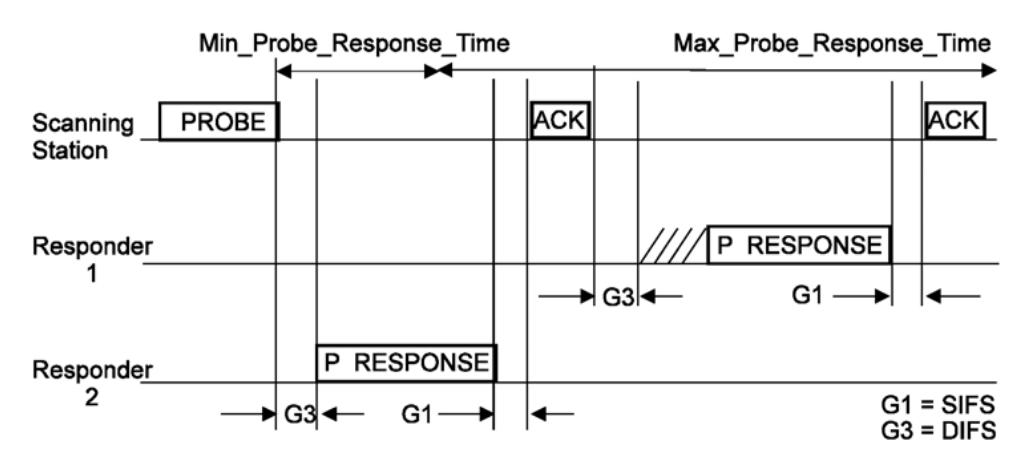
\includegraphics[width=0.9\textwidth]{images/activescan.png}
  \caption{Ablaufdiagramm eines aktiven Scan, aus \cite{ieee2012active}.}
  \label{fig:activescan}
\end{figure}


\section{Reichweite von 802.11}
\label{ch:phase1:sec:rangewlan}
Um die Intervallzeit für die Lokalisierung festzulegen, muss die Reichweite von 802.11 im Tunnel bestimmt werden.
Für die Tests wurde ein \emph{LN-862} Access Point von der Firma Lancom zur Verfügung gestellt.
Dieser wurde am hinteren Ende einer Tunnelbohrmaschine in der Tunnelbaustelle Rastatt montiert.\\
Der Durchmesser des Bahntunnels beträgt 9 Meter, das Ende der Tunnelbohrmaschine befand zum Zeitpunkt der Messungen circa 2 Kilometer weit im Tunnel.\\
Der AP konnte aufgrund des geringen Platzangebots und den wenigen zur Verfügung stehenden Steckdosen nicht frei platziert werden.
Er wurde deshalb unter der ersten stählernen Treppe platziert, diese beeinträchtigt natürlich das Signal.
Da es aber üblich ist, IT-Gerätschaften, wie die derzeit verwendeten Bluetooth-Basisstationen, in Metallboxen zu verstauen um sie vor äußeren Einflüssen zu schützen, ist eine gewisse Abschirmung durchaus realitätsnah.
Die Platzierung des AP ist auf Abbildung \ref{fig:tunnelmark} eingezeichnet.\\
Abbildung \ref{fig:applacement} zeigt den \emph{LN-862} hinter der Treppe.

\begin{figure}[h]
  \centering
	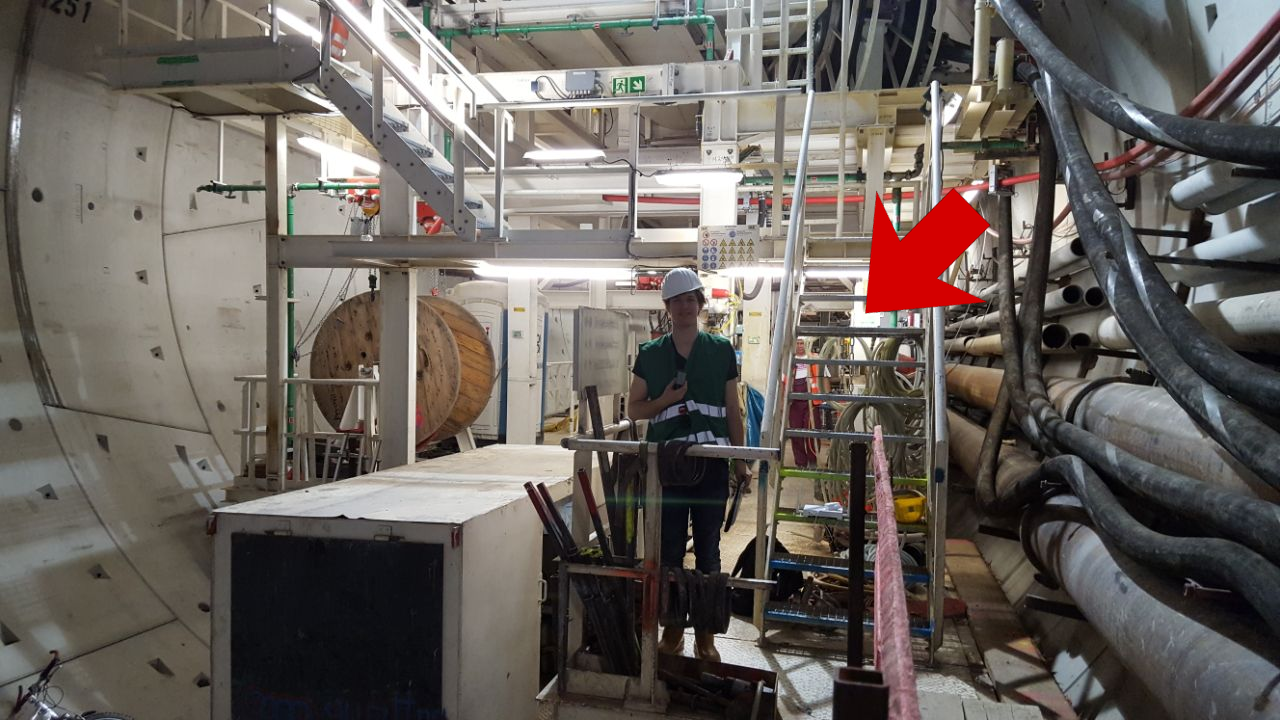
\includegraphics[width=\textwidth]{images/tunnelmark.png}
  \caption{Ende der Tunnelbohrmaschine, Pfeil markiert Platzierung des Access Point hinter der Treppe.}
  \label{fig:tunnelmark}
\end{figure}

\begin{figure}[h]
  \centering
	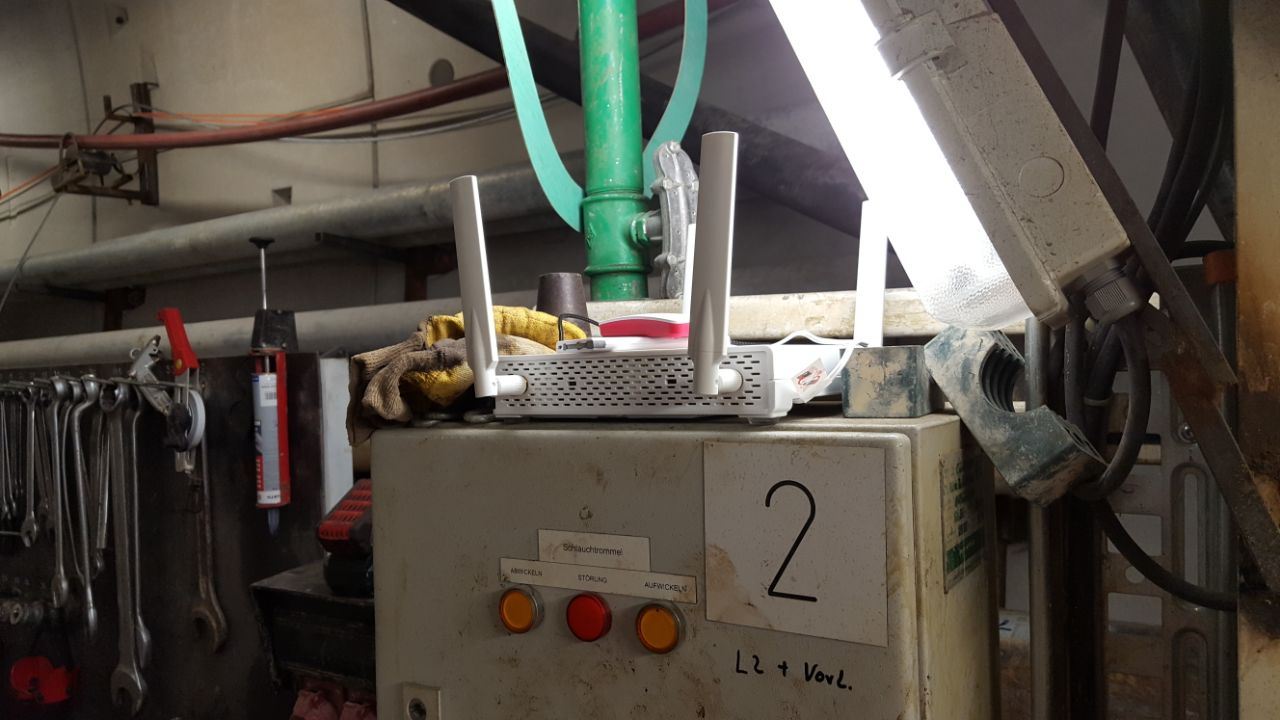
\includegraphics[width=\textwidth]{images/applacement.jpg}
  \caption{\emph{LN-862} im Tunnel, darauf liegt ein \emph{Raspberry Pi Zero W}.}
  \label{fig:applacement}
\end{figure}

\subsection{Methodik}
Die Reichweite wurde in zwei Richtungen geprüft.
Zum einen in Richtung des bereits fertig gebohrten Tunnels, hier blockiert nur wenig Stahl das Signal. 
Lediglich die Treppe, unter der der AP montiert wurde, stellt ein Hindernis dar.
Zum anderen wurde die Reichweite in Richtung des Vortriebs geprüft.
Dabei stellen eine stählerne Zwischendecke und große Container Hindernisse dar.
Die zwei Messtrecken werden in Abbildung {fig:rangewlan} skizziert.

\begin{figure}[h!]
  \centering
	\includegraphics[width=\textwidth]{images/rangewlan.eps}
  \caption{Messtrecken zur Festellung der Reichweite von 802.11.}
  \label{fig:rangewlan}
\end{figure}

Außerdem wird die Abschirmung durch ein Gehäuse getestet, dazu wurde eine stabile Plastikbox verwendet.\\
Für die Messung wurde der Körper zwischen mobile Einheit und Basisstation gebracht und eine mobile Einheit wurde dann als "{}außer Reichweite"{} angesehen, wenn versendete Pakete der mobilen Einheit nicht mehr bei der Basisstation ankamen.
In jedem Fall war es möglich durch das Entfernen des körperlichen Hindernisses wieder eine Verbindung herzustellen.\\
Zur Bestimmung der Distanz wurden die \emph{Tübbinge} verwendet, dies sind Schalungselemente im Tunnel.
Im Tunnel Raststatt sind diese fortlaufend nummeriert und genau zwei Meter breit, die Messungen sind deshalb ebenfalls in zwei Meter Schritten angegeben.

\subsection{Ergebnisse}
Tabelle \ref{table:rangewifi} zeigt die Ergebnisse für die zwei verwendeten ESP8266 Module.
Es wurde jeweils mit und ohne Gehäuse gemessen und in jede der beiden beschriebenen Richtungen.
Wenige Hindernisse bezeichnet dabei die Richtung des bereits fertig gebohrten Tunnels, viele Hindernisse die Richtung des Vortriebs.

\begin{table}[h]
	\centering
	\caption{Sendereichweite WLAN-basierter mobiler Einheiten}
	\label{table:rangewifi}
	\begin{tabular}{p{3.5cm}|p{3cm}|p{3.5cm}|p{3cm}}
		Verwendetes Modul & Aufbau & Strecke & Maximale Sendereichweite \\
		\hline
		ESP-12S & Offen & Wenige Hindernisse & 84m \\
		ESP-12S & In Gehäuse & Wenige Hindernisse & 74m \\
		ESP-12S & Offen & Viele Hindernisse & 26m \\
		ESP-12S & In Gehäuse & Viele Hindernisse & 30m \\
		\hline
		ESP-12F & Offen & Wenige Hindernisse & 88m \\
		ESP-12F & In Gehäuse & Wenige Hindernisse & 88m \\
		ESP-12F & Offen & Viele Hindernisse & 32m \\
		ESP-12F & In Gehäuse & Viele Hindernisse & 32m \\
	\end{tabular}
\end{table}


\subsection{Bewertung}
\label{ch:Reichweite:sec:bewertung}
Das ESP-12F Modul hatte in jedem der vier Testszenarien eine höhere Reichweite als das ESP-12S, es ist daher im weiteren Verlauf zu bevorzugen.\\
Für Mitarbeiter im Tunnel kann von einer Maximalgeschwindigkeit von $30\ $km/h ausgegangen werden, diese wird durch Schienen- oder Lastkraftfahrzeuge erreicht. 
Um die gemessenen 88 Meter bei 30 km/h zu durchqueren benötigte ein Mitarbeiter circa 10,5 Sekunden, bei einem Sendeintervall von zehn Sekunden finden demnach zwei Sendevorgänge beim durchqueren des Einflussbereichs eines APs statt.
Da eine zuverlässige Erkennung von Bereichswechseln gefordert wurde, sollte das Sendeintervall jedoch konservativer gesetzt werden, eine Halbierung auf fünf Sekunden ist daher für eine zuverlässige Erkennung sinnvoll.
\\
Für die Teststrecke mit vielen Hindernissen wurden geringere Reichweiten gemessen, eine solche Teststecke findet sich aber nur auf der Tunnelbohrmaschine, welche nur zu Fuß begangen werden kann. 
Geht man von einer maximalen Bewegungsgeschwindigkeit von 10 km/h für eine laufende Person aus durquerte diese in fünf Sekunden 14 Meter, also deutlich weniger als die gemessenen 32 Meter.\\





\section{WiFi-LLS-Implementierung}
\label{ch:phase1:sec:wifills}
Die mobile Einheit des WiFi-LLS Systems führt alle 5 Sekunden einen \emph{Scan} aus, kodiert die Ergebnisse in XML und versendet sie an den Ortungsserver \cite{chen2007design}.
Da der Fokus dieser Arbeit auf dem Energieverbrauch liegt, werden für die Referenzimplementierung einer mobilen WiFi-LLS-Einheit die Kodierung in XML durch eine simple String Kodierung ersetzt und die Ergebnisse werden über UDP an den Ortungsserver übermittelt. 
Damit wird der Overhead einer TCP-Verbindung vermieden.\\
Zunächst muss das Tag dem Netzwerk beitreten (\emph{Join}), einen \emph{Scan} ausführen und ein UDP-Paket versenden.
Der Ablauf eines \emph{Scans} wird in Abbildung \ref{fig:activescan} gezeigt, dieser Vorgang muss für jeden nicht überlappenden Kanal durchgeführt werden.\\
Da die \emph{Scan}-Funktion des ESP8266 Arduino Core es nicht erlaubt den RSSI zu einem AP auszulesen muss \texttt{user\_interface.h} importiert und die \emph{Scan}-Funktion der SDK direkt verwendet werden.
Um den Energieverbrauch weiter zu reduzieren, soll der ESP möglichst viel Zeit in Energiesparzuständen verbringen.
Der tiefste Schlafzustand, der dennoch eine Aufrechterhaltung der WLAN-Verbindung erlaubt ist der \texttt{light\_sleep}. 
Er wird vom ESP8266 automatisch aufgerufen, wenn er keine Aufgaben zu erledigen hat.
Er kann aber auch manuell aufgerufen werden, beides wurde getestet.\\
Einige Parameter können gewählt werden. 
Die Intervallzeit bestimmt, wie oft der ESP aktiv ist und damit auch wie viel Energie er verbraucht.
Die Intervallzeit wird entsprechend der Untersuchung der Reichweite auf fünf Sekunden gesetzt.
Des Weiteren kann theoretisch die Zahl der \emph{gescannten} Kanäle gewählt werden. 
Da sich die Einflussbereiche der APs in einem WLAN-Netzwerk üblicherweise überlappen, ist es aber sinnvoll diese über die vier überlappungsfreien Kanäle zu verteilen. 
Eine Implementierung, die nur einen Kanal \emph{scannt} tritt deshalb nur außer Konkurenz an.\\
Im Folgenden findet eine Voruntersuchung des Energieverbrauchs statt.
Tabelle \ref{table:llsconsumption} zeigt den gemessenen Energieverbrauch der Implementierungen in Arduino und C, jeweils mit und ohne manuell aufgerufenen \texttt{light\_sleep} und eine Implementierung, die nur einen Channel \emph{scannt}.
Für die Tests wurde das Adafruit Feather Huzzah ESP8266 verwendet, es wurde mit 5 Volt aus einer USB-Powerbank mit Energie versorgt, der Verbrauch wurde mit einem dazwischen geschalteten TM103 USB-Power-Meter der Marke Muker gemessen. 
Jeder Versuch wurde mindestens eine Stunde durchgeführt.
Wurde in dieser Zeit der Verbrauchswert von 10 mAh nicht überschritten, wurde der Versuch verlängert, da der TM103 den Verbrauch ohne Nachkommastellen anzeigt.\\
Die Werte wurden stationär in einer Mietwohnung in einem fünfstöckigen Wohnhaus und damit nicht unter realen Bedingungen aufgezeichnet.
Unter realen Bedingungen finden durch die Bewegung des Mitarbeiters regelmäßig Reassizationen statt, im Gegenzug liefert ein \emph{Scan} in einem Tunnel weniger Ergebnisse als in einem Wohnhaus.


%TODO Abstand Tabellenüberschrift
\begin{table}[h]
	\centering
	\caption{Energieverbrauch WiFi-LLS-artiger Tags}
	\label{table:llsconsumption}
	\begin{tabular}{p{3cm}|p{2.2cm}|p{1.5cm}|p{2cm}|p{2cm}|p{2cm}}
		SDK & manueller \texttt{light\_sleep} & Kanäle & Versuchs-dauer in Stunden & Gesamt-verbrauch in mAh & $\varnothing$ Verbrauch in mA  \\
		\hline
		Arduino Core & Nein & alle & 1 & 22 & 22 \\
		Arduino Core & Ja & alle & 1 & 21 & 21 \\
		ESP Open SDK & Nein & alle & 1 & 19 & 19 \\
		ESP Open SDK & Ja & alle & 1 & 19 & 19 \\
		\hline
		ESP Open SDK & Ja & einer & 2 & 13 & 6,5 \\
	\end{tabular}
\end{table}

Die Tests zeigen, dass die Programmierung mit der ESP Open SDK einen Vorteil beim Energieverbrauch hat, dieser liegt bei ca 10\%.
Andererseits fällt auf, dass die Reduzierung der \emph{gescannten} Kanäle eine signifikante Senkung des Energieverbrauchs nach sich zieht, die \emph{Scan}-Funktion ist also der Hauptverbraucher.\\
Die Implementierung in C mit manuellem \texttt{light\_sleep} werden in Abschnitt \ref{ch:phase1:sec:powerwifills} genauer untersucht.

%%%%%%%%%%%%%%%%%%%%%%%%%%%%%%%%%%%%%%%%%%%%%%%%%%Abschnittsende








\section{Anpassungen für Bereichsortung}
\label{ch:phase1:sec:anpassungbereich}
Bei WiFi-LLS wird der \emph{Scan} durchgeführt, um den RSSI zu nahen Access Points zu erhalten und dann auf dem Ortungsserver die Position der mobilen Einheit mit einer Trilateration zu berechnen.
Im Tunnel sind oft nur ein bis zwei APs in Reichweite, außerdem wird eine Bereichsortung als ausreichend angesehen. \\
Werden die APs geschickt den Bereichen zugeordnet, reicht das Wissen um einen nahen AP, um die mobile Einheit einem Bereich zuzuordnen.
Da der mobilen Einheit die MAC-Adresse seines Netzzugangs bekannt sein muss, kann dies als Ortungsinformation verwendet werden.
Der Wechsel zwischen zwei Access Points wird exemplarisch in Abbildung \ref{fig:reassociation} dargestellt.

\begin{figure}[h!]
  \centering
	\includegraphics[width=\textwidth]{images/reassociation.eps}
  \caption{Vorgang von Assoziation und Reassoziation.}
  \label{fig:reassociation}
\end{figure}

Die MAC-Adresse des Access Points wird nun zusammen mit der eigenen MAC-Adresse als Identifikator als String kodiert und per UDP an den Ortungsserver versendet.\\
Tabelle \ref{table:naiveconsumption} zeigt den gemessen Verbrauch der Implementierungen in Arduino und C, jeweils mit und ohne manuell aufgerufenen \texttt{light\_sleep}.

\begin{table}[h]
	\centering
	\caption{Energieverbrauch der Bereichsortungstags}
	\label{table:naiveconsumption}
	\begin{tabular}{p{3cm}|p{2.2cm}|p{1.7cm}|p{2.5cm}|p{2.5cm}}
		SDK & manueller \texttt{light\_sleep} & Versuchs-dauer in Stunden & Gesamt-verbrauch in mAh & $\varnothing$ Verbrauch in mA \\
		\hline
		Arduino Core & Nein & 1 & 14 & 14 \\
		Arduino Core & Ja & 3 & 21 & 7 \\
		ESP Open SDK & Nein & 2 & 12 & 6 \\
		ESP Open SDK & Ja & 2 & 11 & 5,5 \\
	\end{tabular}
\end{table}

Der Verbrauch liegt wie erwartet unter dem der WiFi-LLS-Implementierung, sogar unter der Implementierung, die nur einen Kanal scannt.
Als weitere Optimierung könnte eine mobile Einheit nur dann senden, wenn eine Reassoziation stattgefunden hat.
Die mangelnde Transportsicherheit von UDP macht dieses Vorgehen jedoch riskant, wenn das Paket verloren geht wird kein Bereichswechsel erkannt.
Um wieder eine begrenzte Transportsicherheit zu erhalten, kann entweder das UDP-Paket mehrfach versendet werden; ohne Reassoziation in einen festen, aber größeren Intervall gesendet werden oder statt eine UDP-Verbindung eine TCP-Verbindung verwendet werden.
Somit ergeben sich neue Testszenarien: Ohne zusätzliche Sicherung, UDP-Paket mehrfach (dreifach) versenden, zusätzliches (30 beziehungsweise 60 Sekunden) Sendeintervall, TCP-Verbindung (offen halten oder nach dem Senden schließen). \\
Da der Verbrauch nun stark von der Anzahl der Reassoziationen abhängt sind im gegebenen, stationären Testszenario keine aussagekräftigen Ergebnisse möglich.
Dennoch sollen die Tests einen Ausgangswert ermitteln, dieser kann als untere Grenze für den Verbrauch einer Implementierung angesehen werden.
Da in den vorherigen Tests die Implementierungen mit der ESP Open SDK verbrauchsärmer waren, wurden alle in Tabelle \ref{table:naiveoptconsumption} gezeigten Implementierungen mit ihr erstellt, der manuelle \texttt{light\_sleep} ist immer aktiv.

\begin{table}[h]
	\centering
	\caption{Energieverbrauch der verbesserten Bereichsortungstags}
	\label{table:naiveoptconsumption}
	\begin{tabular}{p{3.5cm}|p{1.7cm}|p{2.5cm}|p{2.5cm}}
		Transportsicherung & Versuchs-dauer in Stunden & Gesamt-verbrauch in mAh & $\varnothing$ Verbrauch in mA \\
		\hline
		Ohne & 5 & 10 & 2 \\
		Dreifach UDP & 10 & 14 & 1,4 \\
		Zusatzintervall 30s & 13 & 34 & 2,62 \\
		Zusatzintervall 60s & 5 & 8 & 1,6 \\
		TCP (halten) & 10 & 12 & 1,2 \\
		TCP (schließen) & 11 & 12 & 1,09 \\
	\end{tabular}
\end{table}

Der Energieverbrauch sinkt durch das Einsparen von Sendevorgänge deutlich.
In Abschnitt \ref{ch:phase1:sec:powerindirekt} werden die Implementierungen, die eine TCP Verbindung nutzen genauer untersucht.
Diese bieten eine gute Übertragungssicherheit bei geringem Verbrauch.


\section{Untersuchung des Energieverbrauchs}
\label{ch:phase1:sec:energie}
Der Muker TM103 USB-Power-Meter bietet sowohl im Zeit- als auch im Wertebereich nur eine sehr geringe Auflösung.
Stattdessem soll der Verbrauch mit einem INA219 Chip genauer untersucht werden.
Er kann den Verbrauch mit bis zu 333Hz bestimmen und besitzt dabei eine Messgenauigkeit von 99,5\% \cite{texas2015ina}.
Der Stromverbrauch wird über den Spannungsabfall über einen 0,1$\Omega$ Widerstand bestimmt, der verwendete Widerstand besitzt eine Fertigungstoleranz von 1\%.
Die Messgenauigkeit sinkt deshalb auf $99,5\% * 99\% = 98,505\%$. 
Das über $I^2C$ auslesbare Register löst den aktuellen Verbrauch in 0,1 Milliamper Schritten auf, Verbräuche darunter können nicht bestimmt werden.\\
Außerdem wird dieses mal durch den JST-Anschluss für den Akku gemessen, dadurch können eventuelle Ineffizienzen des Lithium-Polymer-Ladeschaltkreises aufgezeichnet werden. 
Jede Messung wurde über eine Stunde durchgeführt.
Abbildung \ref{fig:ina219} zeigt den INA219 integriert auf einer Platine, diese wird für die Messungen verwendet.

\begin{figure}[h!]
  \centering
	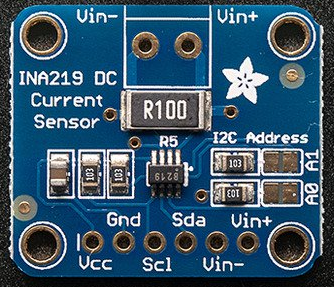
\includegraphics[width=0.5\textwidth]{images/ina219ada.png}
  \caption{INA219, die mit R100 beschriftete Komponente über dem INA219 ist der Messwiderstand. Bild von Adafruit Industries.}
  \label{fig:ina219}
\end{figure}

\subsection{WiFi-LLS}
\label{ch:phase1:sec:powerwifills}
Abbildung \ref{fig:wifills} zeigt den Lastverlauf nach Anschalten der mobilen Einheit für die Implementierung von WiFi-LLS, wenn ein AP zur Verfügung steht. 

\begin{figure}[h!]
  \centering
	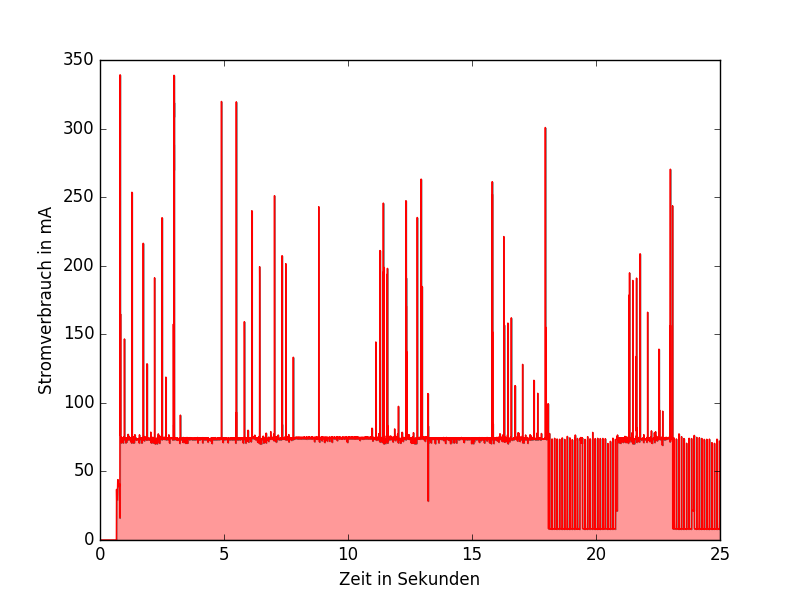
\includegraphics[width=\textwidth]{plots/wifills.png}
  \caption{Lastkurve einer Implementierung von WiFi-LLS.}
  \label{fig:wifills}
\end{figure}

Diese beginnt bei circa einer Sekunde mit dem \emph{Scan}, nachdem sie diesen beendet hat beginnt sie bei 5 Sekunden mit dem \emph{Join}-Vorgang.\\
Der ESP8266 empfängt während des \emph{Join} die gesamte Zeit und verbraucht dabei circa 70 Milliamper, nachdem dieser jedoch abgeschlossen ist synchronisiert er sich mit dem AP und lauscht alle 100ms auf den \emph{Beacon} des AP.
Ist im \emph{Beacon} eine Aufforderung zum Empfangen für den ESP8266 enhalten empfängt er länger um die Nachricht zu erhalten, ein solches Verhalten ist bei circa 19 Sekunden zu erkennen.\\
Bei 12, 17 und 22 Sekunden werden weitere \emph{Scans} ausgeführt, diese stehen im Zentrum der Implementierung, da sie implizit die Position bestimmen.
Die rote Kurve in Abbildung \ref{fig:wifillssendv} zeigt diesen Vorgang genauer, ein \emph{Scan} besteht für jeden gescannten Kanal aus dem Versenden eines \emph{Probe Request} und anschließenden Empfangen der \emph{Probe Responses}. 
Abschließend wird ein Paket an den Ortungsserver versendet und der Chip wechselt wieder in einen Zustand, in dem er periodisch die \emph{Beacons} des AP empfängt.\\

\begin{figure}[h!]
  \centering
	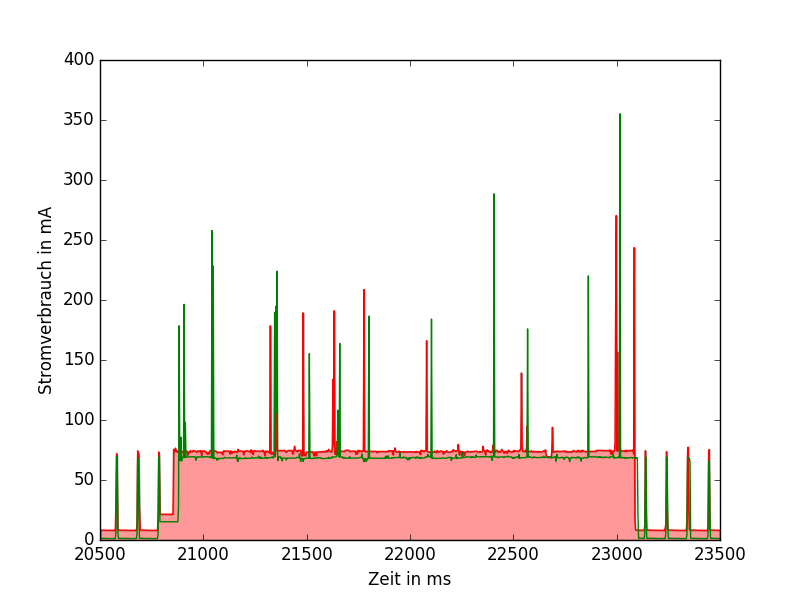
\includegraphics[width=\textwidth]{plots/wifillssendv.png}
  \caption{Lastkurve eines Ortungsvorgangs mit WiFi-LLS.}
  \label{fig:wifillssendv}
\end{figure}

Auffällig ist, dass der Chip circa 8,2 Milliamper verbraucht wenn er nicht empfängt, dagegen gibt das Datenblatt des ESP8266 nur einen Verbrauch von 0,9 Milliamper an.
Das Experiment wurde deshalb mit einem ESP-12F Modul wiederholt, welches nicht auf einem ESP8266 Feather verbaut war. 
Dabei zeigte sich, dass dieses in der selben Situation nur 1,2 Milliamper verbraucht.
Die Lastkurve des einzelnen ESP-12F Modul ist in Abbildung \ref{fig:wifillssendv} grün dargestellt.
Daraus lässt sich schließen, dass die zusätzlichen Komponenten auf dem ESP8266 Feather 7 Milliamper Vebrauch erzeugen, dies ist im Zuge der Laufzeitoptimierung nicht tragbar.\\
Zusätzlich wurde die Implementierung von WiFi-LLS mit nur einem \emph{gescannten} Kanal geprüft.
Abbildung \ref{fig:wifills1chsend} zeigt den verkürzten Ortungsvorgang.
Da nur ein Kanal \emph{gescannt} wird, wird nur ein \emph{Probe Request} versendet.
Nach Empfangen der Antworten wird ein Paket an den Ortungsserver gesendet und der ESP8266 wechselt wieder in den Zustand des periodischen Empfangens.\\

\begin{figure}[h!]
  \centering
	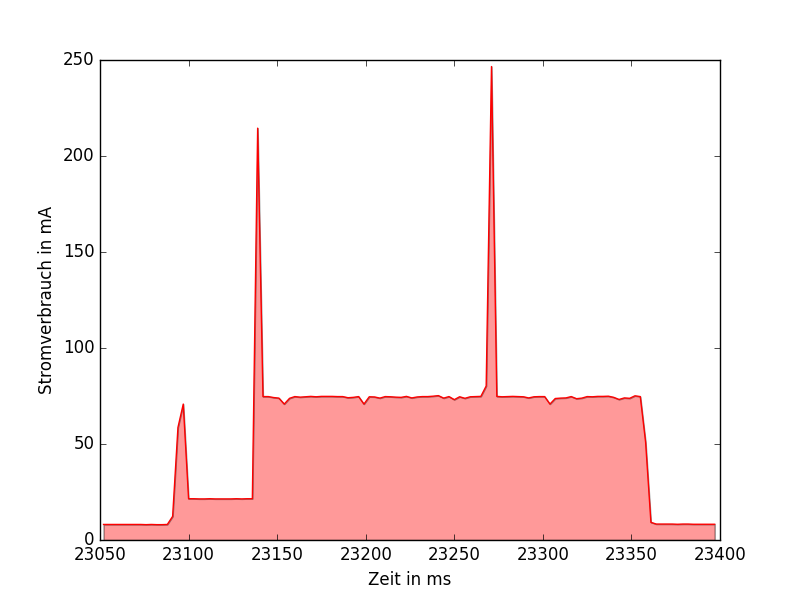
\includegraphics[width=\textwidth]{plots/wifills1chsend.png}
  \caption{Lastkurve des Ortungsvorgangs mit einem gescannten Kanal.}
  \label{fig:wifills1chsend}
\end{figure}

Tabelle \ref{table:wifillsina} listet den durchschnittlichen Verbrauch der Einheiten über eine Stunde.
Die Stromversorgung der Einheiten wurden circa eine Sekunde nach Beginn des Experiments angeschaltet, anschließend treten keine Veränderungen mehr auf.

\begin{table}[h!]
	\centering
	\caption{Energieverbrauch mobiler Einheiten mit WiFi-LLS Implementierung}
	\label{table:wifillsina}
	\begin{tabular}{p{3.5cm}|p{5cm}|p{2.5cm}|p{2.5cm}}
		Hardware & Programm & $\varnothing$ Verbrauch in mA & Laufzeit in Stunden\\
		\hline
		ESP8266 Feather & WiFi-LLS alle Kanäle & 42,2 & 33,2\\
		ESP-12F & WiFi-LLS alle Kanäle & 36,5 & 38,3\\
		ESP8266 Feather & WiFi-LLS ein Kanal & 18,7 & 74,9\\
		ESP-12F & WiFi-LLS ein Kanal & 11,4 & 122,8\\
	\end{tabular}
\end{table}

Um die finale Laufzeit zu bestimmen muss die Kapazität des Akkus bekannt sein.
Ein 1400mAh Lithium-Polymer-Akku wurde als leicht genug angesehen, um um den Hals getragen werden zu können.
Die Laufzeiten in Tabelle \ref{table:wifillsina} wurden für diesen 1400mAh Akku mit 1400 mAh / X mA = Y h bestimmt.



\subsection{Indirekte Bereichsortung}
\label{ch:phase1:sec:powerindirekt}
Abbildung \ref{fig:tcphold} zeigt den Lastverlauf nach Anschalten der mobilen Einheit für die Implementierung für Bereichsortung mit aufrecht erhaltener TCP-Verbindung, wenn ein AP zur Verfügung steht. 
Der Beginn des Lastverlaufs ist dem der WiFi-LLS-Implementierung ähnlich, es werden ebenfalls \emph{Scan} und \emph{Join} durchgeführt.
Da jedoch nur für das Event einer vollständigen (Re-)Assoziation gesendet wird bleibt der ESP8266 anschließend im Zustand des periodischen Empfangens von \emph{Beacons}.
Diese wird nur von den \emph{Keep-Alive-Paketen} unterbrochen, welche alle 30 Minuten versendet werden.\\

\begin{figure}[h!]
  \centering
	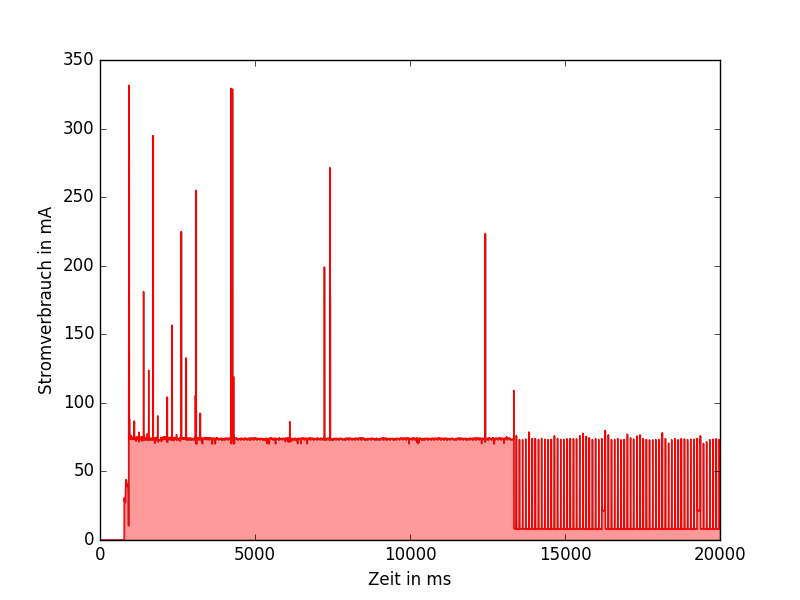
\includegraphics[width=\textwidth]{plots/tcphold.png}
  \caption{Lastkurve einer Implementierung indirekter Bereichsortung, welche eine TCP Verbindung offen hält.}
  \label{fig:tcphold}
\end{figure}

Für die Implementierung mit anschließendem Abbau der TCP-Verbindung kommen zusätzliche Pakete direkt nach dem Versenden der Assoziationsinformation an den Ortungsserver hinzu, dafür entfallen die \emph{Keep-Alive-Pakete}.
Abbildung \ref{fig:tcpdisco} zeigt dieses Verhalten.\\

\begin{figure}[h!]
  \centering
	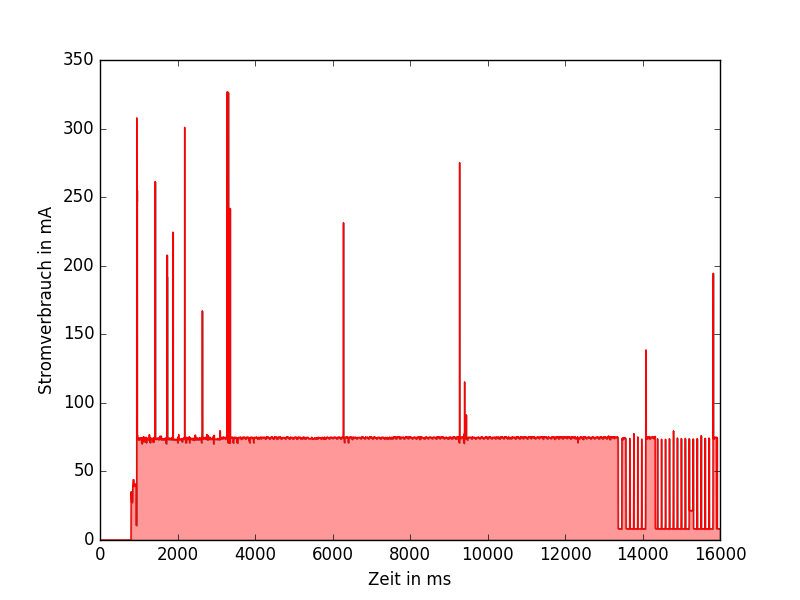
\includegraphics[width=\textwidth]{plots/tcpdisco.png}
  \caption{Lastkurve einer Implementierung indirekter Bereichsortung, welche eine TCP Verbindung nach dem Senden abbaut.}
  \label{fig:tcpdisco}
\end{figure}

Auch diese Implementierungen wurden sowohl mit einem ESP8266 Feather, als auch mit einem einzelnen ESP-12F Modul getestet, die Ergebnisse sind in Tabelle \ref{table:associatonina} zu finden.

\begin{table}[h!]
	\centering
	\caption{Energieverbrauch mobiler Einheiten mit Bereichsortung}
	\label{table:associatonina}
	\begin{tabular}{p{3.5cm}|p{5cm}|p{2.5cm}|p{2.5cm}}
		Hardware & Programm & $\varnothing$ Verbrauch in mA & Laufzeit in Stunden\\
		\hline
		ESP8266 Feather & Bereichsortung TCP Verbindung halten & 15,5 & 90,3\\
		ESP-12F & Bereichsortung TCP Verbindung halten & 8,8 & 159,1\\
		ESP8266 Feather & Bereichsortung TCP Verbindung schließen & 15,4 & 90,9\\
		ESP-12F & Bereichsortung TCP Verbindung schließen & 8,8 & 159,1\\
	\end{tabular}
\end{table}

\subsection{Kein AP in Reichweite}
Bisher wurden die besonderen Bedingungen des Tunnels nicht berücksichtigt.
Für den ESP-12F wurde nur eine Reichweite von 88 Metern gemessen, aber auch für die zukünftige Situation mit einem Access Point alle 250 Meter wäre eine Reichweite von 125 Metern notwendig um eine durchgehende Abdeckung für den ESP-12F zu erreichen.
Außerdem besteht vor dem Portal des Tunnels ein großer Arbeitsbereich ohne WLAN-Abdeckung.\\
Es muss deshalb auch die Situation ohne erreichbaren AP geprüft werden.
Die Untersuchung dazu zeigt unmittelbar, dass der ESP8266 sofort den nächsten \emph{Scan} startet, nachdem der vorherige nicht erfolgreich war.
Ist also kein AP erreichbar \emph{scannt} der ESP8266 durchgehend, sein Verbrauch ist entsprechend hoch.\\
Als Optimierung kann der nicht erfolgreiche \emph{Scan} als Event verarbeitet und der ESP8266 in den \texttt{deep\_sleep} versetzt werden.
Abbildung \ref{fig:noap} zeigt das Profil des Energieverbrauchs eines einzelnen ESP-12F Moduls, wenn kein AP des angefragten Netzwerks verfügbar ist.
Die rote Kurve zeigt dabei die Implementierung aus dem vorherigen Abschnitt, die Implementierung, die den fehlgeschlagenen \emph{Scan} abfängt ist in grün dargestellt.

\begin{figure}[h!]
  \centering
	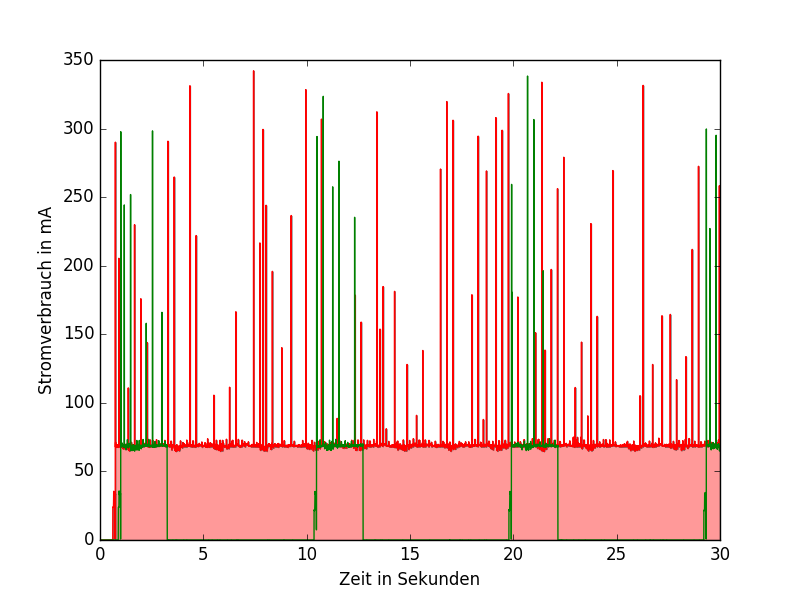
\includegraphics[width=\textwidth]{plots/noap.png}
  \caption{Lastkurve einer Implementierung indirekter Bereichsortung, wenn kein Access Point verfügbar ist.}
  \label{fig:noap}
\end{figure}

Die Ergebnisse dere Messungen ohne verfügbaren AP sind in Tabelle \ref{table:noapina} gelistet.
Auch mit der Optimierung liegt der Verbrauch der 
Auch mit der Optimierung liegt der Energieverbrauch fast doppelt so hoch wie der Verbrauch wenn ein AP verfügbar ist.

\begin{table}[h!]
	\centering
	\caption{Energieverbrauch mobiler Einheiten mit Bereichsortung (ohne verfügbaren AP)}
	\label{table:noapina}
	\begin{tabular}{p{3.5cm}|p{5cm}|p{2.5cm}|p{2.5cm}}
		Hardware & Programm & $\varnothing$ Verbrauch in mA & Laufzeit in Stunden\\
		\hline
		ESP-12F & Bereichsortung TCP Verbindung schließen & 69,37 & 20,2\\
		ESP-12F & Bereichsortung TCP Verbindung schließen, mit \texttt{deep\_sleep} nach fehlgeschlagenem \emph{Scan} & 17,1 & 81,9\\
	\end{tabular}
\end{table}

